
%     Copyright 2021, Abt Dávid Ottó

%         Szegedi Tudományegyetem
% Természettudományi és Informatikai Kar
%          Informatikai tanszék

% A szakdolgozathoz felhasználtam az alábbi linkeken található sablont:
% https://github.com/szledan/thesis-template

\documentclass[12pt,numbers=noenddot]{report}

\usepackage[a4paper]{geometry}
\usepackage{lmodern}			% Kijelölhető az összes karakter
\usepackage[utf8]{inputenc}		% Ékezetes szavak beviteléhez
\usepackage[hungarian]{babel}	% Magyar nyelv támogatása
\usepackage{fontspec}			% Fontok támogatása
\setmainfont{Nimbus Roman}		% FOSS Times New Roman alternatíva
\usepackage{titlesec}			% Fejlécben lévő cím margójának beállítására
\usepackage{fancyhdr}			% Fej- és láblécek személyreszabása
\usepackage{graphicx}			% Képek
\graphicspath{ {./img/} }
\usepackage{color}				% Színek
\usepackage{xcolor}				% -||-
\usepackage{subfig}
\usepackage{caption}
\captionsetup[figure]{labelsep=colon}
\usepackage{tikz}
\usepackage{float}				% Hogy az ábrák a helyükön maradjanak
\usepackage{wrapfig}			% Kép mellett folyó íráshoz
\usepackage{listings}			% Forráskódok
\usepackage{lastpage}			% Utolsó oldal száma
\usepackage[unicode]{hyperref}	% Linkek
\hypersetup{
	colorlinks,
	citecolor=black,
	filecolor=black,
	linkcolor=black,
	urlcolor=black
}
\usepackage[block=ragged]{biblatex}
\BiblatexHungarianWarningOff
\bibliography{cites}
\DeclareFieldFormat{urldate}{Látogatás:}

\usepackage{amsmath}

\usepackage{multicol}

\usepackage{amssymb} 

\usepackage{verbatim}

% Egyéni színek
\definecolor{codegreen}{rgb}{0,0.6,0}
\definecolor{codegray}{rgb}{0.5,0.5,0.5}
\definecolor{codepurple}{rgb}{0.58,0,0.82}
\definecolor{backcolour}{rgb}{0.95,0.95,0.92}

% Kódrészletek
\lstset{ %
	backgroundcolor=\color{backcolour},
	commentstyle=\color{codegreen},
	keywordstyle=\color{magenta},
	numberstyle=\tiny\color{codegray},
	stringstyle=\color{codepurple},
	basicstyle=\ttfamily\footnotesize,
	breakatwhitespace=false,
	breaklines=true,
	captionpos=b,
	keepspaces=true,
	numbers=left,
	numbersep=5pt,
	showspaces=false,
	showstringspaces=false,
	showtabs=false,
	tabsize=4,
	extendedchars=true
}

% Ábrák számozása
\renewcommand{\thefigure}{\arabic{chapter}.\arabic{figure}}
% Ábrák "ábra" felirata
\addto\captionsmagyar{\renewcommand{\figurename}{{\'a}bra}}

% Tartalomjegyzék elemeinek számozása:
\setcounter{tocdepth}{3}
\setcounter{secnumdepth}{3}

% Margók:
\voffset	-1in
\textwidth	150mm
\topmargin	15mm
\headheight	10mm
\headsep	5mm
\textheight	237mm

% A Word-ös 1.5-ös sorköznek ez felel meg
\linespread{1.25}

\begin{document}

\pagestyle{fancyplain}
\fancyhf{}
\renewcommand{\headrulewidth}{0pt}	% Eltűnteti a fejlécben lévő vonalat

\titleformat{\chapter}[display]
{\normalfont\huge\bfseries}{\thechapter. \chaptertitlename}{20pt}{\Huge}
\titlespacing*{\chapter}{0pt}{0pt}{40pt}

\newcommand{\szerzo}{Abt Dávid Ottó}
\newcommand{\cim}{Másodrendű sajátvektor centralitások vizsgálata}

%%%%%%%%%%%%%%%%%%%%%%%%%%%%%%%%%%%%%%%%%%%%%%%%%%%%%%%%%%%%%%%%%%%%%%%%%%%%%%%%
%% Elülső kötéstábla                                                          %%
%%%%%%%%%%%%%%%%%%%%%%%%%%%%%%%%%%%%%%%%%%%%%%%%%%%%%%%%%%%%%%%%%%%%%%%%%%%%%%%%

\newpage
\thispagestyle{empty}
\fancyfoot[C]{}	% Lábléc eltüntetése

\begin{center}

	\vspace*{2cm}

	{\Large\bf Szegedi Tudományegyetem}

	\vspace{.5cm}

	{\Large\bf Informatikai Intézet}

	\vspace*{8.5cm}

	{\Huge\bf SZAKDOLGOZAT}

	\vspace*{7cm}

	{\LARGE\bf \szerzo}

	\vspace*{.6cm}

	{\Large\bf 2022}

\end{center}

%%%%%%%%%%%%%%%%%%%%%%%%%%%%%%%%%%%%%%%%%%%%%%%%%%%%%%%%%%%%%%%%%%%%%%%%%%%%%%%%
%% Címlap                                                                     %%
%%%%%%%%%%%%%%%%%%%%%%%%%%%%%%%%%%%%%%%%%%%%%%%%%%%%%%%%%%%%%%%%%%%%%%%%%%%%%%%%

\newpage
\thispagestyle{plain}

\begin{center}
	\vspace*{.6cm}

	{\Large\bf Szegedi Tudományegyetem}

	\vspace{.5cm}

	{\Large\bf Informatikai Tanszékcsoport}

	\vspace*{3.5cm}

	{\LARGE\bf \cim}

	\vspace*{3.2cm}

	{\Large Szakdolgozat}

	\vspace*{3.5cm}

	\large
	\begin{tabular}{c@{\hspace{4cm}}c}
	\emph{Készítette:}						&\emph{Témavezető:}\\
	\textbf{\szerzo}						&\textbf{Dr. Vinkó Tamás}\\
	programtervező informatikus BSc				&egyetemi docens\\
	hallgató								&
	\end{tabular}

	\vspace*{3.5cm}

	\Large {
		Szeged\\
		\vspace{2mm}
		2022
	}
\end{center}

%%%%%%%%%%%%%%%%%%%%%%%%%%%%%%%%%%%%%%%%%%%%%%%%%%%%%%%%%%%%%%%%%%%%%%%%%%%%%%%%
%% Üres oldal                                                                 %%
%%%%%%%%%%%%%%%%%%%%%%%%%%%%%%%%%%%%%%%%%%%%%%%%%%%%%%%%%%%%%%%%%%%%%%%%%%%%%%%%

\newpage
\thispagestyle{plain}
\mbox{}

%%%%%%%%%%%%%%%%%%%%%%%%%%%%%%%%%%%%%%%%%%%%%%%%%%%%%%%%%%%%%%%%%%%%%%%%%%%%%%%%
%% Feladatkiírás                                                              %%
%%%%%%%%%%%%%%%%%%%%%%%%%%%%%%%%%%%%%%%%%%%%%%%%%%%%%%%%%%%%%%%%%%%%%%%%%%%%%%%%

\chapter*{Feladatkiírás}
\setcounter{page}{1}	% A lapszámláló újrainicializálása
\fancyfoot[R]{\thepage}
\addcontentsline{toc}{section}{Feladatkiírás}

TODO

%%%%%%%%%%%%%%%%%%%%%%%%%%%%%%%%%%%%%%%%%%%%%%%%%%%%%%%%%%%%%%%%%%%%%%%%%%%%%%%%
%% Tartalmi összefoglaló                                                      %%
%%%%%%%%%%%%%%%%%%%%%%%%%%%%%%%%%%%%%%%%%%%%%%%%%%%%%%%%%%%%%%%%%%%%%%%%%%%%%%%%

\chapter*{Tartalmi összefoglaló}
\addcontentsline{toc}{section}{Tartalmi összefoglaló}

\subsubsection*{A téma megnevezése}

\cim

\subsubsection*{A megadott feladat megfogalmazása}

TODO

\subsubsection*{A megoldásmód}

TODO

\subsubsection*{Alkalmazott eszközök, módszerek}

A fejlesztés a \textit{VSCodium} szövegszerkesztő segítségével
zajlott python nyelven, a \textit{NetworkX, NumPy, Matplotlib} és egyéb 
matematikai függvénykönyvtárak használatával. A program számára minta adatok
a \href{https://networkrepository.com/index.php}{Netwrok Repository} weboldalról
lettek letöltve.


\subsubsection*{Elért eredmények}

Egy könnyen kezelhető parancssori alkalmazás, amely tetszőleges gráf 
másodrendű sajátvektor centralitásainak vizsgálatára, összehasonlítására, 
valamint a feltételeknek megadott gráf keresésére alkalmas.

\subsubsection*{Kulcsszavak}

gráf, mátrix, tenzor, sajátérték, centralitás, másodrendűség, NetworkX

%%%%%%%%%%%%%%%%%%%%%%%%%%%%%%%%%%%%%%%%%%%%%%%%%%%%%%%%%%%%%%%%%%%%%%%%%%%%%%%%
%% Tartalomjegyzék                                                            %%
%%%%%%%%%%%%%%%%%%%%%%%%%%%%%%%%%%%%%%%%%%%%%%%%%%%%%%%%%%%%%%%%%%%%%%%%%%%%%%%%

\renewcommand{\contentsname}{Tartalomjegyzék}
\tableofcontents

%%%%%%%%%%%%%%%%%%%%%%%%%%%%%%%%%%%%%%%%%%%%%%%%%%%%%%%%%%%%%%%%%%%%%%%%%%%%%%%%
%% Bevezetés                                                                  %%
%%%%%%%%%%%%%%%%%%%%%%%%%%%%%%%%%%%%%%%%%%%%%%%%%%%%%%%%%%%%%%%%%%%%%%%%%%%%%%%%

\chapter{Bevezetés}
\addcontentsline{toc}{section}{Bevezetés}
\pagestyle{fancy}

A technológia és az internet fejlődésével nagymértékben megnőtt az emberi 
interakciók száma a különböző online hívás- és chatszolgáltatásoknak, valamint
közösségi médiai platformoknak köszönhetően. Sokkal több emberrel lépünk
kapcsolatba minden nap, mint néhány évtizeddel ezelőtt.

Nem csak az online emberi kapcsolatok mennyiségében történt meg ez a hirtelen
növekedés az utóbbi harminc évben, hanem például a számítógép hálózatok esetén 
is: ma már több mint 10 milliárd eszköz csatlakozik az internetre és kommunikál 
egymással, ami több, mint ahány ember él jelenleg a Földön.

Ezeknek az interakcióknak a formalizálásához, tárolásához, illetve
a rajtuk végzett számításokhoz újfajta modellekre illetve módszerekre volt 
szükség. Itt gyakran nem magukon az entitásokon van a hangsúly, hanem a köztük
létrejött kapcsolatokon. Az ilyen fajta adatok leírására talán a legalkalmasabb
eszköz egy gráf.

Egy gráfnak sok triviális tulajdonsága van, mint például a fokszáma, éleinek 
száma, illetve utóbiak aránya, amivel egyszerű, de látványos kimutatásokat lehet
készíteni. Azonban magas szintű, komplex kérdések megválaszolásához, 
vizsgálatokhoz nem elegendő ezeket az atomi tulajdonságokat kielemezni. 
Például egy baráti társaságban ki az összetartó kapocs? Az, aki a legtöbb embert
közvetlenül ismeri? Az akit a legtöbben ismernek? Az aki ha kiesne a társasából,
akkor sok olyan ember lenne, akinek nincs közös ismerőse?

Sokan a mesterséges intelligencia felől, mélytanulással, neuronhálókkal 
közelítik meg az efféle problémákat. Azonban ezek a módszerek gyakran 
feketedobozként viselkednek, nehéz velük konkrét tulajdonságokat kinyerni egy 
gráfból.

Egy másik megközelítés a centralitások használata. Ez nem olyan elhíresült 
kifejezés manapság, mint az AI, de komoly feladatok elvégzésében nyújtanak 
segítséget, mint például a Google keresésekben a találatok relevanciájának 
kiszámításában.
A centralitás gyakorlatilag egy gráf csúcsaihoz értékeket rendel. Ennek is 
vannak triviális változatai, mint például a fokszámcentralitás, ami minden 
csúcshoz a fokszámát rendeli, azonban ennél sokkal összetettebb, 
akár kettőnél több csúcs kapcsolatát magába foglaló tulajdonságok is léteznek, 
ezeknek a vizsgálatával foglalkozunk a továbbiakban.

%%%%%%%%%%%%%%%%%%%%%%%%%%%%%%%%%%%%%%%%%%%%%%%%%%%%%%%%%%%%%%%%%%%%%%%%%%%%%%%%
%% Alapfogalmak                                                               %%
%%%%%%%%%%%%%%%%%%%%%%%%%%%%%%%%%%%%%%%%%%%%%%%%%%%%%%%%%%%%%%%%%%%%%%%%%%%%%%%%

\chapter{Alapfogalmak}
\addcontentsline{toc}{section}{Bevezetés}
\pagestyle{fancy}

\section{Gráf}

Egy gráf definiálható egy $G=(V,E)$ párként, ahol V a gráf csúcsainak, E az 
éleinek halmaza. Az E halmaz V-beli elempárokat tartalmaz. 
($E \subseteq V \times V$)

Ez a matematikai struktúra alkalmas különböző entitások közti bináris kapcsolatok 
tárolására. Ezek lehetnek akár egy szociális médiai platform felhasználói közti 
ismerettségek, vagy egy internetes enciklopédia kulcsszavai közti összefüggések. 
A gráfok ezen tulajdonságát használja ki például a \textit{neo4j} nevű gráf 
adatbázis kezelő rendszer is.

\section{Mátrix}
A mátrix egy kétdimenziós listaként képzelhető el, ami nem csupán egy $m * n$ 
elemet tároló struktúra, hanem az elemek elhelyezkedésének köszönhetően jóval 
több információt tárol mint egy $m * n$ elemű halmaz.

\section{Gráf ábrázolások, mátrix}
A gráfokat ábrázolására a két legnépszerűbb adatszerkezet a szomszédsági lista, 
illetve a szomszédsági mátrix.

A másodrendű sajátvektor centralitások vizsgálatához a szomszédsági mátrixokat 
fogjuk használni, mivel mátrixokon jóval könnyebb az ezekhez szükséges 
műveleteket elvégezni mint láncolt listákon.

A szomszédsági mátrix egy $n \times n$-es mátrix, ahol $n$ a gráf csúcsainak 
száma. Az $m$-edik sor $n$-edik eleme megadja, hogy a gráf $m$-edik és 
$n$-edig csúcsa közt vezet-e él.


\pagebreak

\section{Sajátérték, sajátvektor}
A mátrixokat felfoghatjuk egy geometriai transzformációként amit egy vektoron 
végzünk el. Például az $\textbf{A}$ mátrix a $\vec{v}$ vektort az alábbiak 
szerint módosítja:

$$
\textbf{A} \vec{v} = \vec{w}
$$

$$
{
	\begin{bmatrix}
		a & b \\
		c & d \\
	\end{bmatrix}
}
{
	\begin{bmatrix}
		x \\
		y \\
	\end{bmatrix}
}
=
{
	\begin{bmatrix}
		a*x+b*y \\
		c*x+d*y \\
	\end{bmatrix}
}
$$

\vspace{1cm}

A transzformáció irányát és mértékét a sajátvektor és a sajátérték jellemzi.
Definíció szerint $A$ mátrix $v$ sajátétvektora és $\lambda$ sajátértéke 
közt az összefüggés: $$A \lambda = v \lambda$$


\section{Centralitás}
A gráfok atomi tulajdonságain (pl.: van-e él két csúcs között) kívül sok 
értékes információ kinyerhető különböző metrikákkal. Például a csúcsok 
"fontosságának" egy kimutatására szolgálnak a centralitások, amik egy sorrendet 
képeznek a gráf pontjai közt. 

A legegyszerűbb centralitás a fokszám centralitás, ami az adott csúcs fokszáma 
szerint képez sorrendet.


\noindent
\begin{minipage}[c]{0.4\linewidth}

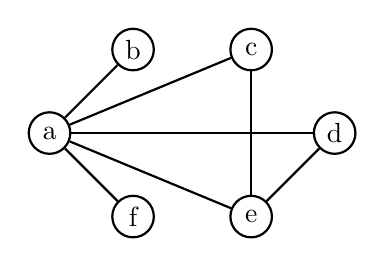
\begin{tikzpicture}[node distance=15mm, inner sep=0pt, minimum size=15pt, 
		thick, main/.style = {draw, circle}]
	\node[main] (1) {a};
	\node[main] (2) [above right of=1] {b};
	\node[main] (3) [right of=2] {c}; 
	\node[main] (4) [below right of=3] {d};
	\node[main] (5) [below left of=4] {e}; 
	\node[main] (6) [left of=5] {f};
	\draw (1) -- (2);
	\draw (1) -- (3);
	\draw (1) -- (4);
	\draw (1) -- (5);
	\draw (1) -- (6);
	\draw (3) -- (5);
	\draw (4) -- (5);
\end{tikzpicture}

\end{minipage}
% \columnbreak
\noindent
\begin{minipage}[c]{0.2\linewidth}

\hspace{0.5cm}
$\rightarrow$

\end{minipage}
% \columnbreak
\begin{minipage}[c]{0.2\linewidth}

\begin{align}
	\begin{bmatrix}
		deg(a)\\
		deg(b)\\
		deg(c)\\
		deg(d)\\
		deg(e)\\
		deg(f)
	\end{bmatrix}
	=
	\begin{bmatrix}
		5\\
		1\\
		2\\
		2\\
		3\\
		1
	\end{bmatrix}
\end{align}

\end{minipage}

\vspace{0.5cm}

A ábrán szereplő 6 pontú gráfhoz egy 6 hosszúságú vektort rendelt, 
melynek elemei az egyes csúcsok fokszámával egyeznek meg.

A fokszám centralitás kiszamítható gráfot leíró $n \times n$ szomszédsági 
mátrix valamint egy $n$ elemű, egyesekből álló vektor szorzataként:

\begin{align}
	\begin{bmatrix}
		0 & 1 & 1 & 1 & 1 & 1 \\
		1 & 0 & 0 & 0 & 0 & 0 \\
		1 & 0 & 0 & 0 & 1 & 0 \\
		1 & 0 & 0 & 0 & 1 & 0 \\
		1 & 0 & 1 & 1 & 0 & 0 \\
		1 & 0 & 0 & 0 & 0 & 0 \\
	\end{bmatrix}
	*
	\begin{bmatrix}
		1\\
		1\\
		1\\
		1\\
		1\\
		1
	\end{bmatrix}
	=
	\begin{bmatrix}
		5\\
		1\\
		2\\
		2\\
		3\\
		1
	\end{bmatrix}
\end{align}


\section{Tenzor}

Egy skalár egy szám, egy $n$ elemű vektort $n$ rendezett érték, egy 
$n \times m$-es mátrix $n*m$ számstruktúra tárolására képes. 
Ezeket a matematikai fogalmakat általánosíthatjuk a tenzorokkal. 
A skalár egy nullad-, a vektor egy első-, a mátrix pedig egy másodrendű tenzornak 
tekinthatő.

Amiért igazán fontos behozni a tenzor fogalmát az az, hogy nem állunk meg a 
másodrendűségnél, léteznek magasabb rendű tenzorok is. Például egy 
$3 \times 3 \times 3$-as tenzor 27 elemből áll, és felfogható egy három 
dimenziós tömbként.


%%%%%%%%%%%%%%%%%%%%%%%%%%%%%%%%%%%%%%%%%%%%%%%%%%%%%%%%%%%%%%%%%%%%%%%%%%%%%%%%
%% Másodrendű sajátvektor centralitások                                       %%
%%%%%%%%%%%%%%%%%%%%%%%%%%%%%%%%%%%%%%%%%%%%%%%%%%%%%%%%%%%%%%%%%%%%%%%%%%%%%%%%

\chapter{Másodrendű sajátvektor centralitások}


\section{Elsőrendű centralitás}

A korábban látott fokszám centralitás egy elsőrendő centralitás volt,
mivel fokszám az adott csúcshoz kapcsolódó élek számát jelenti,
egy él pedig két csúcs között teremt kapcsolatot. 

Az elsőrendű centralitások kiszámításához elég volt egy mátrixszorzást 
végrehajtani egy vektoron, hiszen a mátrix felfogható egy kétdimenziós tömbként
is, aminek az $A[i][j]$-edig eleme jellemzi az összefüggést az $i$-edik és 
$j$-edik csúcs között.


\section{Másodrendű centralitás}

A másodrendű centralitás ezzel szemben csúcshármasok közti kapcsolatok alapján 
fogja jellemezni a gráfot. Három-három csúcs viszonyának tárolására a mátrixok 
nem elegendőek, harmadrendű tenzorok viszont igen.
Ezt fogjuk felhasználni a következőkben.


\section{Általános sajátvektor modell}

A másodrendű centralitások számításához egy operátorra lesz szükség, 
amely végrehajtra a megfelelő leképezést.

Egy \boldmath{$T$}\unboldmath $\in \mathbb{R}^{n \times n \times n}$ 
tenzorhoz és egy $p$ valós paraméterhez definiálunk egy \boldmath{$T_p$}
\unboldmath $: \mathbb{R}^n \rightarrow \mathbb{R}^n$ operátort,
ami egy $n$ elemű vektorhoz egy $n$ elemű vektort rendel. 
Az eredményvektor $i$-edik elemét a következőképp kaphatjuk meg:

$$\boldsymbol{T_p}(\boldsymbol{x})_i = \sum_{j,k=1}^n \boldsymbol{T}_{ijk} 
\mu_p(x_j,x_k)$$

ahol $\mu_p(x_j,x_k)$ a hatványközép, azaz:

$$\mu_p(x_j,x_k) = \left(\frac{|a|^p+|b|^p}{2}\right)^{1/p}$$


Ahhoz, hogy hatékonyan vizsgálatokat tudjunk végezni a különböző 
centralitásokon szükségünk lesz egy egységes kiszámítási módra.

Legyen $\alpha \in \mathbb{R}: 0 \leq \alpha \leq 1$ skalár, ami az első- 
és másodrendűség lineáris kombinációjának az arányát adja meg,
illetve legyen $M \in \mathbb{R}^{n \times n}$ nemnegatív elemekből álló, 
a gráfhoz tartozó négyzetes mátrix, valamint $\boldsymbol{T} \in 
\mathbb{R}^{n \times n \times n}$ szintén nemnegatív elemegkből álló, 
gráfot jellemző tenzor. Ekkor definiálhatunk egy $\mathcal{M}: 
\mathbb{R}^n \rightarrow \mathbb{R}^n$ operátort, hogy

$$\mathcal{M}(\boldsymbol{x}) = \alpha M \boldsymbol{x} + (1-\alpha) 
\boldsymbol{T}_p(\boldsymbol{x})$$

\noindent
Ekkor az első- és a másodrendű centralitás $i$-edik csúcsbeli értéke $x_i 
\geq 0$ ahol x kielégíti a sajátérték problémát:
$$\mathcal{M}(\boldsymbol{x}) = \lambda \boldsymbol{x}$$

\noindent
$\alpha$ megfelelő megválasztásával kiszámíhatjuk csak az elsőrendű 
centrailtás értéket $(\alpha = 1)$, vagy csak a másodrendű centralitás 
értéket $(\alpha = 0)$, illetve a kettő súlyozott kombinációját is.


\section{$M$ és $\boldsymbol{T}$ megválasztása}

Az $M$ mátrix az elsőrendű összetevője, tehát valamilyen elsőrendű 
információt kellene elkódolnia. 
Erre egy kézenfekvő lehetőség a szomszédsági mátrix.

A fontosabb szerepet pedig a $\boldsymbol{T}$ tenzor tölti be, hiszen ez 
tartalmazza a vizsgálandó másodrendű kapcsolatokat.

\subsection*{Bináris háromszögtenzor}

A másodrendű kapcsolatoknak egyik legjobb példája, ha az adott három csúcs egy
háromszöget zár be, azaz páronként össze vannak kötve egy-egy éllel.
Ennek az elkódolásához egy olyan tenzorra van szükségünk, amelynek az első 
dimenziója szerinti $i.$, második dimenzója mentén $j.$, harmadik dimenziója
mentén $k.$ elem akkor $1$, ha a gráfnak az $i., j., k.,$ csúcsa egy háromszöget
alkot, különben $0$:

\begin{equation}
	(\boldsymbol{T}_B)_{ijk} = 
		\begin{cases}
			1 & \text{ha} ~ i, j, k ~ \text{csúcsok között páronként szerepel él} \\
			0 & \text{különben}
		\end{cases}
\end{equation}

\pagebreak

\subsection*{Random séta háromszögtenzor}

A random séta háromszögtenzor egy normalizált változata a bináris 
háromszögtenzorznak, azzal a trükkel, hogy ha $i, j, k$ egy háromszöget alkot,
akkor nem $1$ lesz a tenzor adott értékének az eleme, hanem a $(j,k)$ élet
tartalmazó háromszögek számának a reciproka.
Egy adott $(j,k)$ élet tartalmazó gráfbeli csúcsháromszögek számát könnyen ki 
lehet számolni a szomszédsági mátrix alapján:

$$\Delta(j,k) = (A \circ A^2)_{jk}$$

\noindent
ahol a $\circ$ művelet a mátrixok elenkénti szorzását jelöli.

A kapott tenzor ezek alapján:

\begin{equation}
	(\boldsymbol{T}_W)_{ijk} = 
		\begin{cases}
			\frac{1}{\Delta(j,k)} & \text{ha} ~ i, j, k ~ \text{csúcsok között páronként szerepel él} \\
			0 & \text{különben}
		\end{cases}
\end{equation}

Fontos megemlíteni, hogy $\boldsymbol{T}_W$ jól definiált, hiszen ha 
$i, j, k$ csúcsok háromszöget alkotnak, akkor $\Delta(j,k)$ legalább $1$.


\subsection*{Klaszterező-együttható háromszögtenzor}

Egy másik megközelítés lehet, ha a csúcshármasoktól nem várjuk el, hogy 
alkossanak háromszöget, hanem csak annyi, hogy egy "szeletben" vegyenek részt,
azaz legalább kettő élhez kapcsolódjanak.
Tehát az $i$ csúcsot érintő háromszögek számának reciproka helyett az $i$ 
csúcsból kiinduló irányítatlan szeletek számának reciprokát vesszük alapul.

Ha $d_i$ az $i.$ csúcs fokszámát jelöli, akkor $d_i(d_i-1)$ szorzat pont a 
keresett értéket adja meg. Ezek alapján a tenzor:

\begin{equation}
	(\boldsymbol{T}_C)_{ijk} = 
		\begin{cases}
			\frac{1}{d_i(d_i-1)} & \text{ha} ~ i, j, k ~ \text{csúcsok között páronként szerepel él} \\
			0 & \text{különben}
		\end{cases}
\end{equation}

Ezesetben is $\boldsymbol{T}_C$ jól definiált, mivel ha 
$i, j, k$ csúcsok háromszöget alkotnak, akkor $d_i(d_i-1)$ legalább $2$.

\pagebreak

\subsection*{Local closure háromszögtenzor}

Az utolsó tenzor, amit vizstgálni fogunk ismét egy másik megközelítése a 
másodrendű kapcsolatoknak.
Most az adott csúcsból kiinduló kettő hosszúságú utakat vesszük figyelembe a
számításnál a háromszögek illetve a szeletek keresése helyett.
Ezt megkaphatjuk úgy, hogy összeadjuk az adott csúccsal szomszédos csúcsok 
fokszámát, és kivonjuk belőle az adott csúcs fokszámát.
Vagy pedig összeadjuk az adott csúccsal szomszédos csúcsok fokszámánál egyel
kisebb értékeket:

$$w(i) = \sum_{j \in N(i)} d_j - d_i = \sum_{j \in N(i)} (d_j - 1)$$

ahol $N(i)$ az $i$-vel szomszédos mezők halmazát jelöli.

Ebben az esetben a tenzor a következő:

\begin{equation}
	(\boldsymbol{T}_L)_{ijk} = 
		\begin{cases}
			\frac{1}{w(i)} & \text{ha} ~ i, j, k ~ \text{csúcsok között páronként szerepel él} \\
			0 & \text{különben}
		\end{cases}
\end{equation}

Amely szintén jól definiált, hiszen ha $i, j, k$ háromszöget alkot, akkor 
biztosan létezik nullánál több kettő hosszúságú $i$-ből kiinduló út a gráfban.

%%%%%%%%%%%%%%%%%%%%%%%%%%%%%%%%%%%%%%%%%%%%%%%%%%%%%%%%%%%%%%%%%%%%%%%%%%%%%%%%
%% Implementáció                                                              %%
%%%%%%%%%%%%%%%%%%%%%%%%%%%%%%%%%%%%%%%%%%%%%%%%%%%%%%%%%%%%%%%%%%%%%%%%%%%%%%%%

\chapter{Implementáció}

\section{Fejlesztői környezet}

A programot GNU/Linux operácios rendszer alatt VSCodium-ban fejlesztettem 
(Visual Studio Code nyílt forráskódú és szabad változa). A python nyelvet 
választottam, ami egy széles körben elterjedt szkriptnyelv, egyszerű 
szintaxissal, és sokrétű matematikai függvénykönyvtárakkal rendelkezik,
így a célnak tökéletesen megfelel.

A NetworkX a használt csomagok közül a legfontosabb, a gráfok beolvasását,
kezelését, illetve a rajtuk elvégzett műveleteket is támogatja. Ezen kívül
említésre méltó még a NumPy és a Pandas, amiket mátrixműveletek kiszámítására
használtam, valamint az argparse, amit parancssori argumentumok beolvasásában 
segített, illetve a Matplotlib, amivel az eredményeket kirajzoltattam.

\section{A program magja}

Ahhoz, hogy gráfok centralitását összehasonlítsuk, először ki kell tudni szamolni őket.
Az első lépés ennek az implementációja volt. Bemenetként egy gráfot kapunk, és az elvárt kimenet a 
$\mathcal{M}(\boldsymbol{x}) = \lambda \boldsymbol{x}$
egyenlet egy közelítő megoldása. 

Az egyenlet kiszámításához egy iterációs módszerre lesz szükségünk, a hatványmódszerre.
Ez az eljárás iteratív lépések segítségével a legnagyobb abszolútértékű sajátértékhez
és a hozzá tartozó sajátvektorhoz ad közelítő megoldást. 
Az algoritmus alapja ez az iteráció:
$$\boldsymbol{y}^{(k)} = A \boldsymbol{x}^{(k)}$$
$$\boldsymbol{x}^{(k+1)} = \frac{\boldsymbol{y}^{(k)}}{||\boldsymbol{y}^{(k)}||}$$

ahol az első egyenlet egy mátrix-vektor szorzás, a második pedig ennek a részeredménynek a normált értékét adja meg.
A kiinudlási ($\boldsymbol{x}^{(0)}$) vektor nem lehet merőleges a legnagyobb abszolútértékű sajátértékhez tartozó sajátvektorra.

\pagebreak

A mi esetünkben ez a következőképpen néz ki:

$$\boldsymbol{y}^{(k)} = \mathcal{M}(\boldsymbol{x})$$
$$\boldsymbol{x}^{(k+1)} = \frac{\boldsymbol{y}^{(k)}}{||\boldsymbol{y}^{(k)}||}$$

vagyis

$$\boldsymbol{y}^{(k)} = \alpha M \boldsymbol{x} + (1-\alpha) \boldsymbol{T}_p(\boldsymbol{x})$$
$$\boldsymbol{x}^{(k+1)} = \frac{\boldsymbol{y}^{(k)}}{||\boldsymbol{y}^{(k)}||}$$


\section{Az egyenlet paraméterei}

A kiszámítás előtt szükségünk lesz az $\alpha$-ra, az $M$-re, illetve $\boldsymbol{T_p}$-re, és a hozzá szükséges tenzorra.
Alfa egyszerű skalár paraméter, $M$-et, mint szomszédsági mátrixot pedig megkaphatjuk 
a NetworkX \texttt{adjacency\_matrix} nevű függvényével.

A tenzorok előállítását saját függvényekkel oldottam meg. 
Az input itt is egy gráf (NetworkX-es \texttt{Graph} típusban eltárolva),
és hátrom egymásba ágyazott for ciklus tölti fel a háromdimenziós tömbként tárolt tenzorokat.
Ezeke a függvények felépítésükben nagyban hasonlítanak, egyedül a tenzor értékét adó logika tér el.
Itt említést érdemel a NumPy csomag \texttt{ndarray, multiply, matmul} és \texttt{ones} függvényei,
amik sok forciklus megírását spórolták meg, ezzel rövidebbé, és átláthatóbbá téve a kódot.

A $\boldsymbol{T_p}$ operátornak egy háromparaméteres függvényt írtam, ami a tenzort, 
az $\boldsymbol{x}$ vektort, illetve $p$-t kapja inputként. 
A vektort itt egy hagyományos pyhton-os listaként kezeltem.

Még egy fontos paraméter, ami az egyenletben nincs explicit jelölve, az az iterációk száma.
Mivel iterációs módszerről beszélünk, így meg kell adni egy egész értéket is, 
hogy hány iteráció után szeretnénk visszatérni az eredménnyel. Minél tovább iterálunk,
annál pontosabb eredményt kapunk, azonban annál több erőforrást és időt vesz igénybe a program.

$\boldsymbol{x}$ kezdeti értékét eleinte egy random $n$ hosszúságú vektorra állítottam be,
aztán a determinisztikus műkösés miatt áttértem az egyesekből álló vektorra, így 
könnyebb volt a későbbiekben ellenőrizni a program helyességét.


\section{Teszt adatok}

A NetworkX a gráfokkal kapcsolatos függvényeken és eljárásokon kívül 
tartalmaz néhány gráfot is, például Zachary karate klubjának a gráfját.
Én is ezt használom a teszteléshez, illetve a program ezzel számol 
alapértelmezett gráfként, ha nem adunk meg mást.

Egyéb gráfok beszerzésére a \href{https://networkrepository.com/index.php}{Netwrok Repository}
oldalt használtam, ahool több ezer gráf áll rendelkezésre ingyenesen. 
Igyekeztem kisebb fokszámú $(|V|<100)$, de nem triviális gráfokat keresni.


\section{A keretprogram}
A szoftvert egy mérésre, kísérletezésre alkalmas eszközként képzeltem el,
amiben a matematikai számításokon van a hangsúly, nem pedig a felhasználói felületen.
Így a Unix filozófiához hűen egyszerű parancssori alkalmazásban gondolkoztam,
ami ``egy dolgot csinál, de azt jól csinálja''.

A program fejlesztésének első fázisában probléma volt, hogy az aktuális haladást
mindig ki akartam próbálni, esetleg az eredményeket képeken ábrázolni, és aztán
változtatni rajta, újra kipróbálni. Erre kézenfekvő megoldás volt, hogy 
az alkalmazásnak a számításhoz szükséges benemeneti paramétereken kívül 
meg lehessen adni, hogy milyen funkciót végezzen el.
Így ha valami újfajta mérést szerettem volna leimplementálni, akkor elég volt
létrehozni neki egy új funkciót, amit a helyes paraméterezés esetén végrehajt.

\section{Parancssori argumentumok}

A program futtatásához kell egy funkciót megadni parancssori paraméter formájában, 
amivel meghatározzuk, hogy milyen számítást hajtson végre a program. 
Ez az egyetlen kötelező paraméter.

\noindent
Például:

\texttt{python main.py solve}

\noindent
ahol a \texttt{solve} funkciót szeretnénk elvégeztetni a programmal.

Ezen kívül lehetőségünk van a következő paraméterek állítására is:

\begin{itemize}
	\item \texttt{--graph}, röviden \texttt{-g}, a gráf megadására, 
		amin számolni szeretnénk
	\item \texttt{--tensor}, röviden \texttt{-t}, a tenzor(ok) megadására, 
		amivel a másodrendű kapcsolatokat jellemezzük. 
		(Egyes funkciókhoz több tenzort is meg lehet adni.)
	\item \texttt{--alpha}, röviden \texttt{-a}, az egyenlet $\alpha$ paramétere
	\item \texttt{-p} a gráf megadására, az egyenlet $p$ paramétere
	\item \texttt{--num\_iter}, röviden \texttt{-n}, a hatványmódszerben az 
		elvégezendő iterációk szám
	\item \texttt{--treshold}, röviden \texttt{-x}, a \texttt{find-similar} 
		funkciókban az optimális hasonlóság mértéke
\end{itemize}

\noindent
Ezeket a paramétereket, és a hozzájuk tartozó rövid magyarázatot a

\texttt{python main.py --help}

\noindent
utasítással le tudjuk kérdezni.
Példa egy paraméterezésre:

\texttt{python src/main.py --graph input\_graphs/soc-firm-hi-tech.txt --tensor random\_walk --alpha 0.6 -p 2 --num\_iter 15 solve}


%%%%%%%%%%%%%%%%%%%%%%%%%%%%%%%%%%%%%%%%%%%%%%%%%%%%%%%%%%%%%%%%%%%%%%%%%%%%%%%%
%% Funkciók                                                                  %%
%%%%%%%%%%%%%%%%%%%%%%%%%%%%%%%%%%%%%%%%%%%%%%%%%%%%%%%%%%%%%%%%%%%%%%%%%%%%%%%%

\chapter{Funkciók}


\section{Solve}

Az első funkció, amit a program nagyon korai fázisában implementálva lett, 
az a \texttt{solve}, ami gyakorlatilag kiszámítja az általános sajátvektor 
modell egyenletét az kapott paraméterek alapján, hatványmódszer segítségével.
Az eredményvektort a képernyőre írja ki. Az előző oldalon szereplő példa esetén
az output a következő:

\vspace{0.4cm}

\footnotesize
\noindent
% \texttt{
\begin{verbatim}
[0.00840449 0.12371296 0.00840449 0.22103893 0.51571457 0.10745514
	0.06594145 0.38736454 0.20666928 0.25458575 0.11321281 0.26577601
	0.11070488 0.2408121  0.31856498 0.0964164  0.11184042 0.14277145
	0.10582157 0.0454091  0.08996091 0.04470695 0.17091334 0.18363112
	0.05318976 0.07146028 0.03518014 0.05129317 0.003085   0.02035976
	0.01828195 0.00239007 0.00617164]
\end{verbatim}
% }
\normalfont

\section{Compare}

A centralitások vizsgálatának az egyik legkézenfekvőbb formája az 
összehasonlítás. Minden centralitás a gráf valamely jellemzője alapján
felállít egy sorrendet a csúcsok között a hozzájuk rendelt értékekkel.
Ezeknek a sorrendeknek összehasonlításához a Kendall rangkorrelációs 
együtthatót (röviden: Kendall tau) vesszük igénybe, ami egy 
$x \in \mathbb{R}: 0 \leq x \leq 1$
értékkel jellemzi a centralitások eredményeként kapott vektorok hasonlóságát
a sorrendiség szempontjából.

A Kendall tau kiszamításához az \texttt{scipy} csomag \texttt{stats} 
alkönyvtárának a \texttt{kendalltau} függvényét használjuk fel, ami a két 
összehasonlítandó vektort várja paraméterként, és a Kendall rangkorrelációs 
együtthatóval, valamint a p-értékkel tér vissza.

A program képes egyszerre akár kettőnél több tenzorhoz tartozó centrailtás 
összehasonlítására is a \texttt{compare} funkcióval. Az erdmény egy táblázat, aminek első sorában és 
oszlopában szerepelnek az összehasonlított centralitásokhoz tartozó tenzorok 
nevei, az egyes mezőkben pedig az adott sorhoz és oszlophoz tartozó centralitás
korrelációja: a főátló felett a Kendall korrelációs rangegyütthatók, a főátló
alatt a p-értékek.

\noindent
Példa a funkció használatára:

\texttt{python src/main.py compare -t binary -t random\_walk -t clustering\_coefficient -t local\_closure}

\pagebreak

\noindent
Ehhez a bemenethez tartozó eredmény:

\scriptsize
\begin{verbatim}
p_value \ tau              binary  random_walk  clustering_coefficient  local_closure
binary                 1.00000000   0.64349376              0.66131907     0.64349376
random_walk            0.00000009   1.00000000              0.98217469     1.00000000
clustering_coefficient 0.00000004   0.00000000              1.00000000     0.98217469
local_closure          0.00000009   0.00000000              0.00000000     1.00000000
\end{verbatim}
\normalsize

\section{Comparison}

Gyakran ha összehasonlítást szeretnénk elvégezni, nem csak egy adott 
paraméterezéses mérésnek az eredményére vagynk kíváncsi, mint amit az előző
funkció produkál, hanem például több $\alpha$ érték esetén lennénk kíváncsiak
a hasonlóságokra. Erre szolgál a \texttt{comparison} funkció, ami szintén 
a megadott tenzorokhoz tartozó centralitásokat hasonlítja össze, azonban itt 
nem az általunk megadott $\alpha$-ra, hanem $0$-tól, $1$-ig $0.1$-es lépéssel
minden $\alpha$-ra elvégzi az összehasonlítást.

Ez esetben nem lenne célszerű az eredményt a standart outputon megjeleníteni,
így ehelyett inkább egy adatbázisba kerülnek a kapott korrelációs együtthatók.
A célnak tökéletesen megfelel az sqlite adatbázis, hiszen relatíve kevés 
adatot szeretnénk letárolni, és így nem kell semmiféle harmadik féltől 
származó szoftvert telepíteni az adatbázisba íráshoz.

A program a $comparison$ funkció futtatása esetén létrehoz egy táblát az 
adatbázisban - ha az még nem lézetik - és letárolja a gráf nevét, az aktuális 
$\alpha$ értéket, $p$ paramétert, illetve a centralitáspárok tartozó korrelációs
értékeket.

\vspace{0.3cm}

\noindent
Például:

\texttt{python src/main.py comparison -p 2 -t degree -t binary -t random\_walk 
-t clustering\_coefficient -t local\_closure}

\noindent
paraméterezés esetén az adtbázisba a következő adatok kerültek:

\vspace{0.3cm}

\noindent
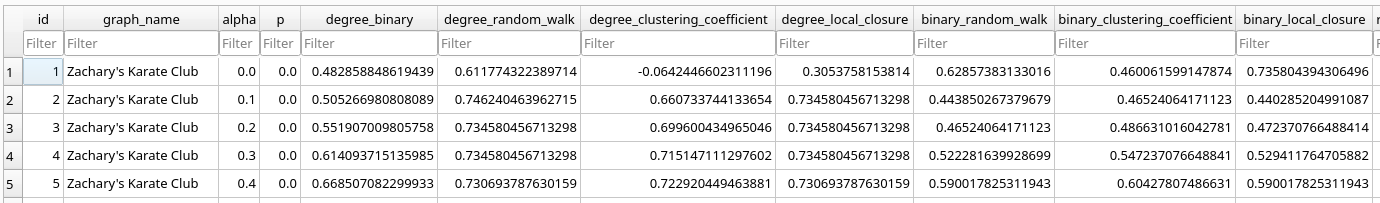
\includegraphics[width=\linewidth]{images/comparison_result.png}

\noindent
A kép részlet, \texttt{sqlitebrowser} alkalmazásban készült.
A korrelációs értékeket tároló mezőket a $tenzor1\_tenzor2$ konvenció alapján 
neveztem el, és a Kendall tau értékét tartalmazzák.

\pagebreak

\section{Find-similar}

\subsection{Keresési probléma}

A program eddigi funkicói arra nyújtottak eszközt, hogy meglévő gráfokon 
végezhessünk méréseket, összehasonlításokat. Azonban gyakran előfordul, hogy
olyanra esetekre vagyunk kíváncsiak, amit még nem láttunk konkrét gráfok esetén.
Tehát nem a centralitás, illetve a centralitások hasonlósága a kérdés, hanem
hogy az általunk kívánt korrelációk milyen gráfok esetén állnak fent.

A \texttt{find-similar} funkciócsalád olyan gráfok keresésére szolgál, ahol
a megadott sajátérték centralitások majdnem megegyeznek. Természetesen a 
triviális gráfokon kívül érdekes ez a kérdés, hiszen például egy teljes gráf
esetén a csúcsoknak nincs kitüntetett szerepük, minden centralitás ugyan azt 
az értéket rendelné a pontokhoz.

\subsection{Kiindulás}
Ahhoz, hogy egy ilyen keresésbe belekezdjünk, szükséges egy kiindulási gráf.
A program eddigi adottságait kihasználva ez szükségszerűen lehet egy parancssori
argumentumként kapott gráf, hiszen több, tetszőleges kezdőállapotból elindítva a 
keresést nagyobb valószínűséggel találunk az elvárásainknak megfelelő, vagy 
legalábbis ahhoz hasonlító gráfot.

\subsection{Algoritmus}
Az alap ötlet az, hogy kiszámítjuk a kezdeti gráfon a sajátérték centralitások
korrelációját, majd változtatunk valamit a gráfon, például egy élet elhagyunk,
vagy egy újat hozzáadunk és megint kiszámítjuk a centralitásokat, és a 
korrelációs együtthatót. Ha az érték jobb (nagyobb) mint az előző, akkor 
az új gráffal megyünk tovább, ha nem, elvetjük a változtatásokat, és újra 
próbálkozunk. 
Ez egy hegymászó algoritmus, azaz kiszámítjuk az adott helyben lévő értéket,
lépünk egyet, kiszámítjuk az új értéket. Ha jobb, megtartjuk. Ha rosszabb,
visszalépünk. Ennek az egyik előnye az, hogy nincs akkora számítás- és időigénye
mintha az összes lehetséges élkombináción végig próbálnánk menni, ami nagyobb 
gráfok esetén szinte kivitelezhetetlen lenne.

\pagebreak

\subsection{Első megvalósítás}
Az algoritmus implementálása során egy hagyományos ciklusos maximuxkeresős 
megoldás volt a legcélszerűbb, ahol nem egy adott strukrúra értékein
végigiterálva történt a keresés, hanem minden iterációban kiszámolásra került
az aktuális gráf centralitásainak korrelációja. Kezdetben ez az előző 
funkciókban már elkészített függvényeket használta. Kettőnél több centralitás
összehasonlítása esetén a korrelációk összegének a maximumát kereste az 
algoritmus.

Minden iterációban 50\% eséllyel kitörölt egy élet a gráfból, 50\% eséllyel 
pedig létrehozott egyett két még nem összkötött csúcs között. Az algoritmus 
természetesen figyelembe vette az aktuális élek számát, tehát például teljes 
gráf esetén biztosan elvesz élet, nem fut hibára.

\subsection{A részeredménynek ábrázolása}
Az algoritmus futása közben kapott gráfokat, illetve a hozzájuk tartozó értéket
nem lenne sem informatív, sem látványos a standard outputon mátrix formában 
megjeleníteni, így arra a következtetésre jutottam, hogy NetworkX és a 
Matplotlib beépített függvényeit kihasználva az egyes gráfokat kirajzoltatom.
A gráfon végbement változtatások kiemelése érdekében a hozzáadott, illetve
elvett csúcsokat a végpontjaikkal együtt zöldre, illetve pirosra színezi
a program, hogy emberi szemmel is könnyen látható legyen, hogy mi változott.

Példa:

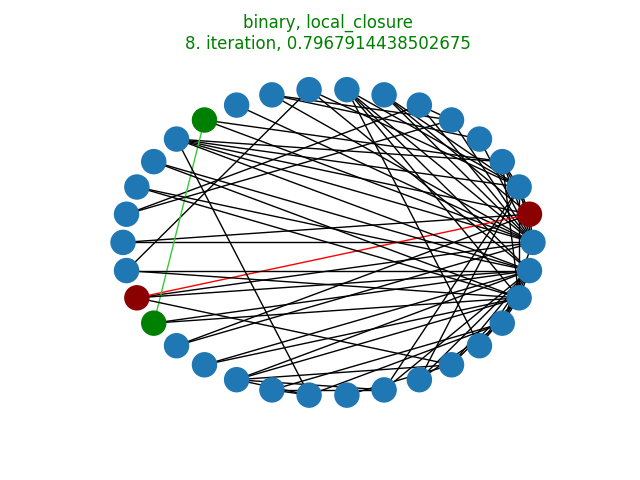
\includegraphics[width=0.9\linewidth]{./images/find_similar_partial_result.png}

Ezen a képen a Bináris háromszögtenzorhoz, illetve a Local closure 
háromszögtenzorhoz tartozó centralitások korrelációja a célfüggvény,
a 8. iterációnál (hegymászó lépésnél) tart az algoritmus, és jelenleg 
~0.7967... a korrelációs együttható értéke.

\subsection{Javítások}

Az első megvalósításban gyakran előfordult, hogy a program egy olyan irányba
vitte a kiinsulási gráfot, hogy annak az éleinek a száma nagymértékben elkezdett
növekedni, vagy épp ellenkezőleg, gyorsan elkezdett csökkenni. 
Az ilyen lefutások gyakran egy kevésbé természetes, jóval inkább triviális 
gráfhoz vezettek, ami nem túl ideális eset számunkra.

E probléma kiküszöbölésére az a megoldás született, hogy az algoritmus 
élszámtartó legyen, azaz mindig pontosan egy élet vegyen el a gráfból 
(továbbra is figyelembe véve azt, hogy a gráf összefüggő maradjon), illetve egy 
még nem létező élet adjon hozzá. Ez a megközelítés egy teljesen új gráf alkotása
helyett a kiindulási gráf éleit rendezi csak át az optimális megoldást keresve.

A másik probléma az volt, hogy kettőnél több centralitás esetén az 
hegymászás nem bizonyult hatékonynak. Kezdetben a program ugyanis a páronként 
összehasonlított centralitások korrelációs együtthatóinak az összegét 
maximalizálta. Ezzel probléma lehet, hogy valamely két centrailtás ténylegesen
közelebb kerül egymáshoz egy részeredmény gráf esetén, de a többivel való
hasonlóság kissé romlik, ami hátráltat az optimális értékhez való eljutásban.

Erre az a megoldás kínálkozott, hogy az egyes centralitások hasonlóságát 
páronként vizsgáljuk, és páronként történik a hegymászás. Ha a korrelációs
együttható eléri az elvárt értéket egy centrailtás pár esetén egy gráfnál,
akkor a következő párral folytatjuk az algoritmust.

Utóbbi megoldással érezhetően megnövekedett az algoritmus sebessége, olyan 
értelemben, hogy hamarabb eljutottunk az elvárt korreláció együttható értékig.

\pagebreak

\subsection{Eredmények}

Az funckió futtatásának eredményei a Karate klub gráf esetén:

\noindent
Kiindulási gráf:

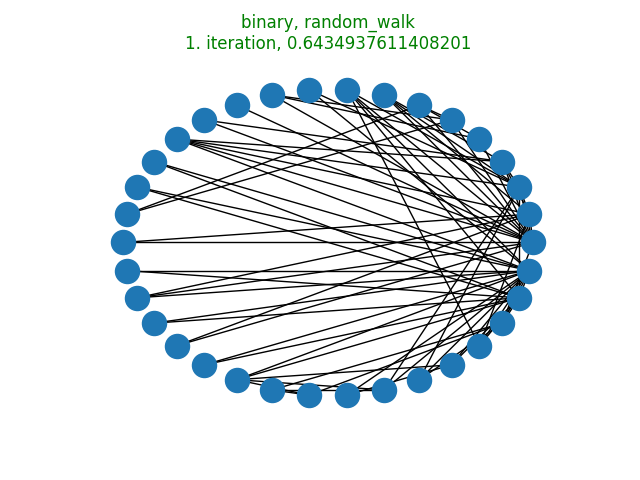
\includegraphics[width=0.85\linewidth]{images/find_similar_start.png}

\noindent
Utolsó iteráció eredménye:

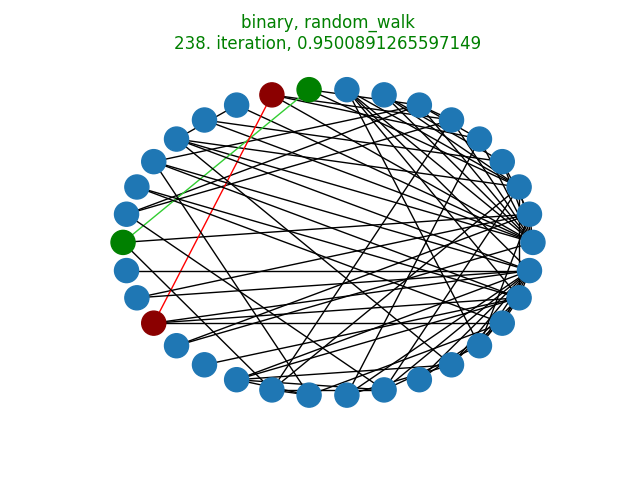
\includegraphics[width=0.85\linewidth]{images/find_similar_end.png}

A program a png képeken kívül az iterációkból készítet gif-et is.

\pagebreak

A kiindulási és az eredményül kapott gráf élszámairól készít hisztogramot is
a szoftver:

\hspace{1cm}

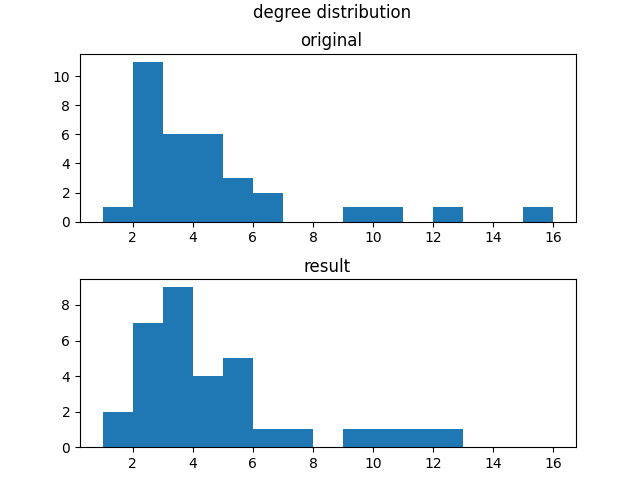
\includegraphics[width=0.95\linewidth]{images/find_similar_histogram.png}

\noindent
valamint scatterplot-ot is:

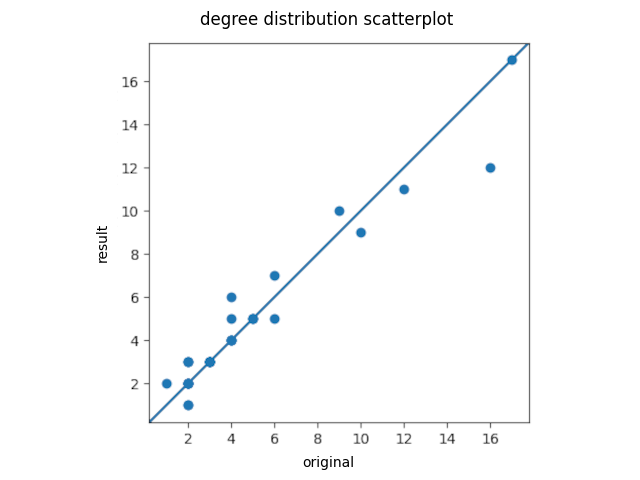
\includegraphics[width=0.95\linewidth]{images/find_similar_scatterplot.png}


A példában használt Karate Klub gráf esetén jól látszik, hogy az eredmény 
gráfban a kiindulásihoz képest az élszámok egyenletesebben oszlanak el, a 
nagyobb fokszámú, illetve a nagyok kis (x<3) fokszámú csúcsok száma csökkent,
több csúcs esett az eredmény gráfban a 3-5 fokszámú csúcsok halmazába.


Egy másik gráf esetén, ami egy csúcstechnológiai cégen belüli kapcsolatokat 
tartalmaz, hasonló eredményeket ért el az algoritmus, itt is egyenletesebb lett 
a csúcsok fokszámainak az eloszlása az eredmény gráf esetén, ahol 97\%-ban 
korrelálnak a sajátvektor centralitások:

\hspace{1cm}

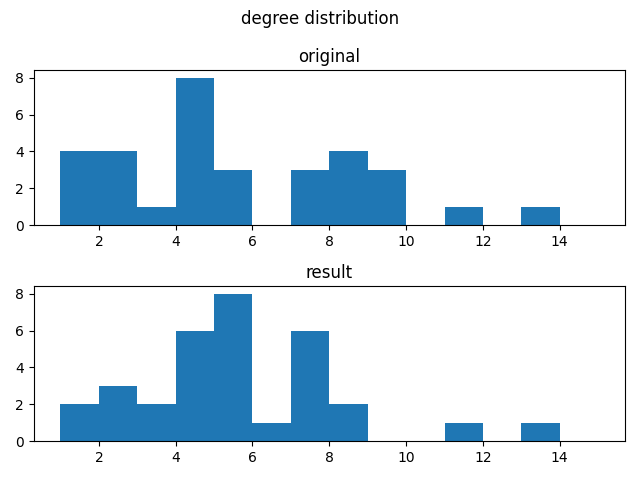
\includegraphics[width=0.8\linewidth]{images/find_similar_histogram2.png}

\hspace{0.5cm}

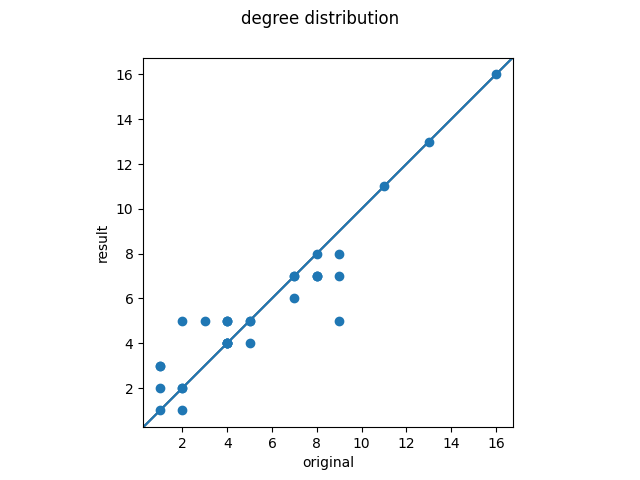
\includegraphics[width=0.8\linewidth]{images/find_similar_scatterplot2.png}




%%%%%%%%%%%%%%%%%%%%%%%%%%%%%%%%%%%%%%%%%%%%%%%%%%%%%%%%%%%%%%%%%%%%%%%%%%%%%%%%
%% Konklúzió                                                                  %%
%%%%%%%%%%%%%%%%%%%%%%%%%%%%%%%%%%%%%%%%%%%%%%%%%%%%%%%%%%%%%%%%%%%%%%%%%%%%%%%%

\chapter{Konklúzió}

A QEMU-ban, illetve VirtualBox-ban végrehajtott tesztelés összességében sikerrel
zajlott. Az alábbiakban részletezem a tesztelt funkciókat, és a kapott
eredményt.

\hfill \break
Végrehajtott tesztek:

\begin{enumerate}
	\item Bootolás QEMU-ban és VirtualBox-ban- sikeres
	\item Megszakítások - működnek
	\item PCI - kilistázza az összes PCI sínnel csatlakoztatott perifériát
	\item Fájlrendszer - felismeri a FAT32-es elsődleges partíciókat, és
	működik a fájlok tartalmának olvasása is
	\item Hálózat (VirtualBox) - működik a kommunikáció a számítógépen nyitott
	netcat-tel, illetve Android eszközön futtatott Debianon lévő netcat-tel is
	\item Soros port (QEMU) - bootoláskor kiírja a boot logot a standard
	outputra, illetve standard inputra bevitt karakterek megjelennek RexOS-en
	\item Párhuzamos port (QEMU) - kiírja a kívánt szöveget
	\item Játékok - hiba nélkül működnek
\end{enumerate}

\noindent Nem lett letesztelve:

\begin{enumerate}
	\item Hálózat (QEMU)
	\item Soros, illetve párhuzamos port (VirtualBox)
	\item Valós hardveren bootolás
\end{enumerate}

\noindent Az operációs rendszerem fejlesztése során rengeteg új információt,
tudást sajátítottam el, és sikerült közelebb kerülnöm a számítógépek működésének
megértéséhez.

%%%%%%%%%%%%%%%%%%%%%%%%%%%%%%%%%%%%%%%%%%%%%%%%%%%%%%%%%%%%%%%%%%%%%%%%%%%%%%%%
%% Irodalomjegyzék                                                            %%
%%%%%%%%%%%%%%%%%%%%%%%%%%%%%%%%%%%%%%%%%%%%%%%%%%%%%%%%%%%%%%%%%%%%%%%%%%%%%%%%

\clearpage
\phantomsection
\addcontentsline{toc}{section}{Irodalom}

\printbibliography

%%%%%%%%%%%%%%%%%%%%%%%%%%%%%%%%%%%%%%%%%%%%%%%%%%%%%%%%%%%%%%%%%%%%%%%%%%%%%%%%
%% Nyilatkozat                                                                %%
%%%%%%%%%%%%%%%%%%%%%%%%%%%%%%%%%%%%%%%%%%%%%%%%%%%%%%%%%%%%%%%%%%%%%%%%%%%%%%%%

\chapter*{Nyilatkozat}
\addcontentsline{toc}{section}{Nyilatkozat}

Alulírott \szerzo, Programtervező Informatikus hallgató, kijelentem,
hogy a dolgozatomat a Szegedi Tudományegyetem, Informatikai Tanszékcsoport
Számítógépes Optimalizálás Tanszékén készítettem, alapszakos diploma megszerzése
érdekében.

\hfill \break
Kijelentem, hogy a dolgozatot más szakon korábban nem védtem meg, saját munkám
eredménye, és csak a hivatkozott forrásokat (szakirodalom, eszközök, stb.)
használtam fel.

\hfill \break
Tudomásul veszem, hogy szakdolgozatomat a Szegedi Tudományegyetem
Informatikai Tanszékcsoport könyvtárában, a helyben olvasható könyvek között
helyezik el.

\vspace*{2cm}

\begin{tabular}{lc}
Szeged, \today
\hspace{2cm} & \makebox[6cm]{\dotfill} \\
& aláírás \\
\end{tabular}

%%%%%%%%%%%%%%%%%%%%%%%%%%%%%%%%%%%%%%%%%%%%%%%%%%%%%%%%%%%%%%%%%%%%%%%%%%%%%%%%
%% Köszönetnyilvánítás                                                        %%
%%%%%%%%%%%%%%%%%%%%%%%%%%%%%%%%%%%%%%%%%%%%%%%%%%%%%%%%%%%%%%%%%%%%%%%%%%%%%%%%

\chapter*{Köszönetnyilvánítás}
\addcontentsline{toc}{section}{Köszönetnyilvánítás}

Szeretném megköszönni a hasznos ismertetőket és kódrészleteket az
\textbf{OSDev wiki szerkesztőinek}, illetve az \textbf{OSDev Discord
szerver tagjainak} útbaigazításait, \textbf{James Molloynak} a kiváló
leírásokkal teli weboldalát, az érthető és szórakoztató
\textit{Write your own Operating System} c. videósorozatot pedig
\textbf{Viktor Engelmannak}. Ez a YouTube videósorozat rengeteget segített nekem
a fejlődésben és az operációs rendszerek működésének megértésében. Egyúttal
szeretném megköszönni a segítségét minden ismerősömnek, aki részt vett az
operációs rendszerem tesztelésben.

\end{document}
